\chapter{Gitflow}

Gitflow è un modello di sviluppo basato su Git, ideato da Vincent Driessen e presentato nel 2010 in un suo celebre post.\footnote{\url{http://nvie.com/posts/a-successful-git-branching-model/}}. Sebbene sia pittosto complicato rispetto ad altri modelli, questo framework fornisce un robusto strumento per la gestione di progetti di grandi dimensioni.

Gitflow assegna ruoli specifici ai diversi branch, specificando quando e come essi debbano interagire tra di loro. Essendo basato su Git gli sviluppatori lavorano in locale e periodicamente effettuano \textit{push} sul repository remoto centrale.

\section{I branch principali}

Nel repository principale si distinguono due rami principali:

\begin{itemize}

\item \textbf{master}, il ramo principale all'interno del quale risiede codice verificato e pronto per essere spedito in \textit{production} e in particolare tutti i suoi nodi corrispondono a \textbf{release} del prodotto, ovvero ad una versione stabile, che può essere marcata o meno con un \textit{tag};

\item \textbf{develop}, il ramo all'interno del quale avviene lo sviluppo vero e proprio del prodotto e dal quale il codice può essere rilasciato, effettuando dunque un \textit{merge} con il ramo master

\end{itemize}

\section{I branch di supporto}

Al livello inferiore dei branch principali troviamo i branch di supporto, che assistono gli sviluppatori nelle operazioni quotidiane di sviluppo. Questi branch, a differenza dei due principali, hanno un tempo di vita limitato e vengono uniti nei rami principali o semplicemente scartati. I tre branch di supporto sono:

\begin{itemize}

\item \textbf{Feature}, che viene creato dal ramo \texttt{develop} ed unito solamente nel medesimo; la loro utilità, come dice la parola stessa, è quella di creare un ramo di sviluppo per un nuovo componente del sistema. Essi normalmente vanno tenuti in locale e non devono essere \textit{pushati} sul repository remoto;

\item \textbf{Release}, che viene creato dal ramo \texttt{develop} ed unito sia nel medesimo che successivamente su \texttt{master}. Questo branch identifica le procedure che vengono istanziate all'atto della release. Quando uno sviluppatore decide di effettuare una release del prodotto apre innanzitutto un brach da \texttt{develop} chiamato \texttt{release-*}, esegue tutte le operazioni di \textit{pre-release}, effettua il merge su \texttt{develop} ed infine il merge su \texttt{master}, marcando il nodo di merge eventualmente con un \textit{tag};

\item \textbf{Hotfix}, che viene creato dal ramo \texttt{master} ed unito prima sia nel medesimo che successivamente su \texttt{develop}. Questi rami derivano dall'immediata necessità di risolvere un \textit{bug} inserito all'interno del ramo master, senza dover effettuare una nuova release. 

\end{itemize}

\begin{figure}[htp]
\centering
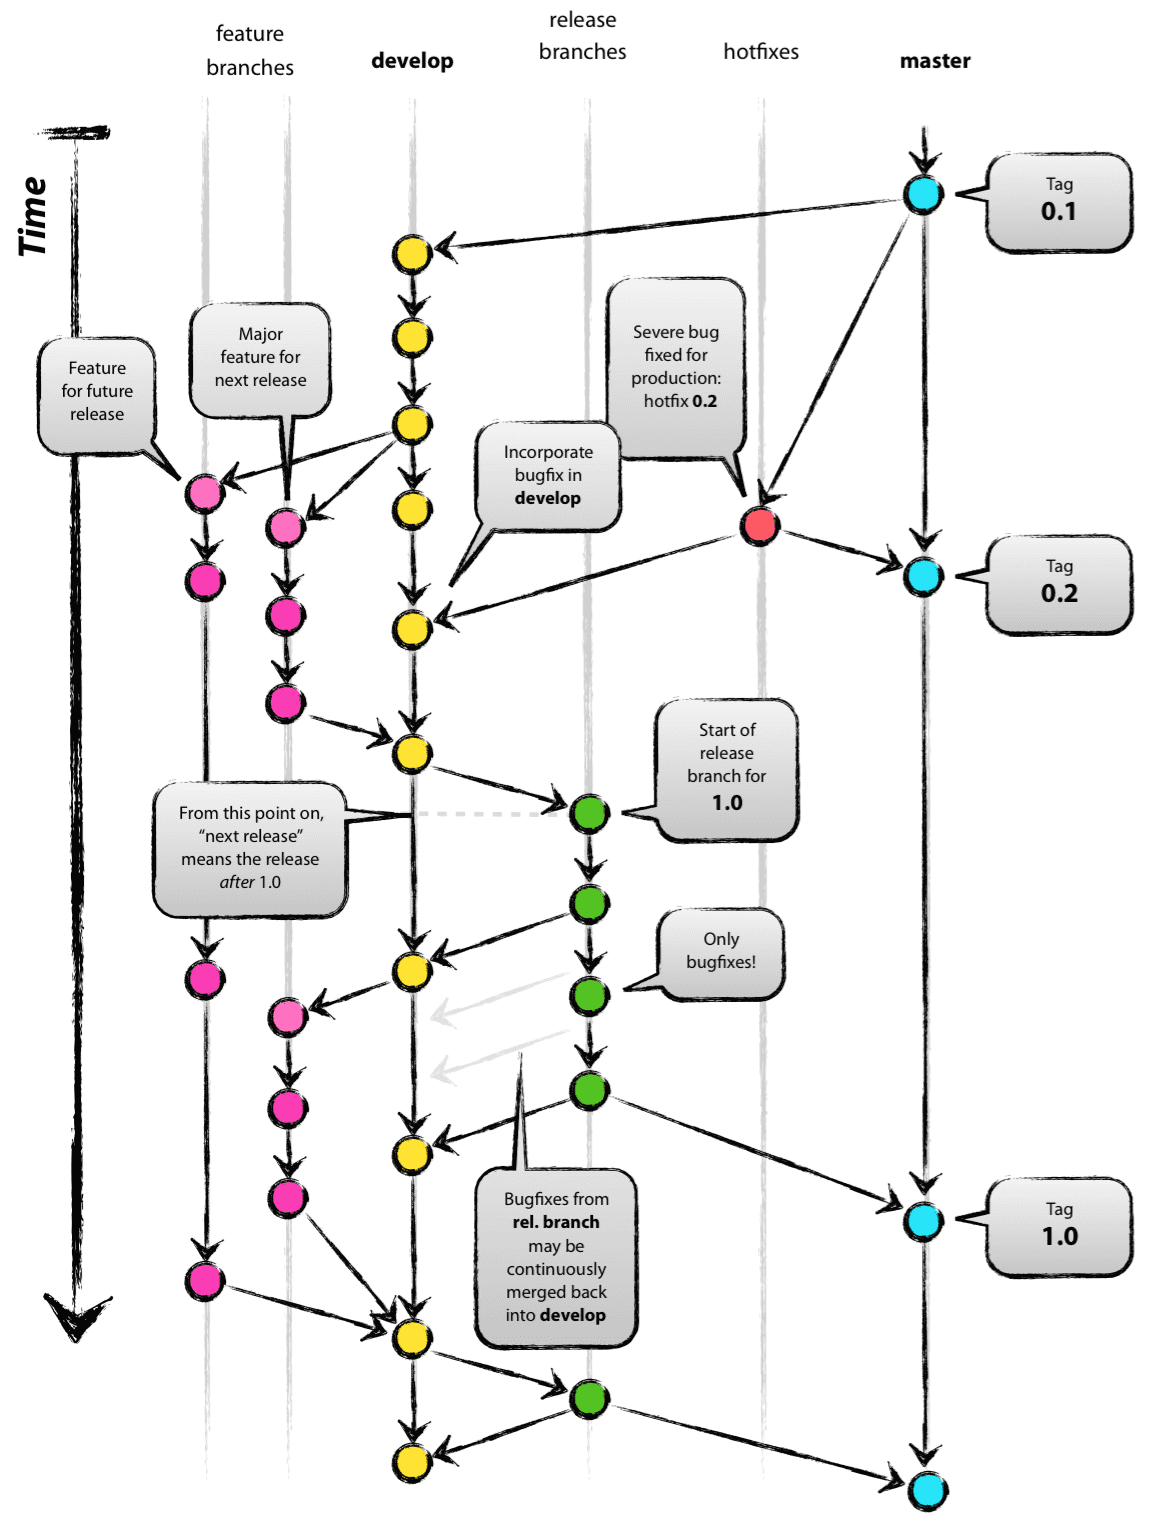
\includegraphics[width=\textwidth/2]{../immagini/git-flow-model}
\caption{Modello Gitflow}
\end{figure}


